
\documentclass[times, 11pt,twocolumn]{article} 
\usepackage{latex8}
\usepackage{times}
\usepackage[ngerman]{babel}
\usepackage{todonotes}
\usepackage[utf8]{inputenc}
\usepackage{graphicx}
\usepackage[hyphens]{url}
\usepackage{mathtools}
\usepackage{amsmath}
\usepackage{amssymb}
\usepackage{esvect}
\usepackage[font=small,labelfont=bf]{caption}

\pagestyle{empty}


\begin{document}

\title{Neuronale Netze in der Videoproduktion}

\author{Laura Anger\\
Technische Hochschule K\"oln \\ Institut f\"ur Medien- und Phototechnik \\  laura.anger@th-koeln.de \\
\and
Vera Brockmeyer\\
Technische Hochschule K\"oln \\ Institut f\"ur Medien- und Phototechnik \\ vera.brockmeyer@smail.th-koeln.de \\
}

\maketitle
\thispagestyle{empty}


\large{\textbf{Zusammenfassung}}\\ \small %\normalsize
\todo[inline, color=yellow]{Vera} 
In der Videoproduktion können die Prozesse sehr Zeit- und Kostenaufwändig sein. Aus diesem Grund gilt es Wege zu finden, einzelne Teilprozesse zu automatisieren und optimieren. Gerade in den Teilbereichen Produktion und Postproduktion gibt es ein enormes Potential für eine Automatisierung. Diese Teilbereiche beschäftigen sich überwiegend mit der Erstellung und Bearbeitung von Bild- und Audiodaten. In den letzten Jahren konnten enorme Erfolge in der Bild- und Audiodatenverarbeitung mit Neuronalen Netzen (NN) erzielt werden. Im besonderen erwiesen sich Faltungsnetze (CNN) als zuverlässige und robuste Automatisierungsalgorithmen. Diese CNN können sowohl zur Klassifikation als auch zur Videodatengenerierung genutzt werden.
\textbf{Es können mit CNN Szenendynamiken aus einem Einzelbild vorhergesagt werden. Zum jetzigen Zeitpunkt ist dies nur mit sehr geringen Auflösung und teilweise fehlerhaft möglich. Die beiden Verfahren \textit{Deep Dream} und \textit{Deep Style} können die Stilsemantik eines Bildes vom Inhalt trennen und auf ein unabhängiges Bild übertragen. \textit{Deep Style} ist ein vielversprechendes Verfahren zur automatischen Stilsynthese, während das \textit{Deep Dream} Verfahren auf Grund mangelnder Reproduzierbarkeit ungeeigneter scheint. Alle vorgestellten Verfahren sind nicht für die Videoproduktion entwickelt worden und werden detailliert beschrieben und auf ihre Tauglichkeit für die professionelle Produktion hin untersucht. }\\


\large{\textbf{Schl\"usselw\"orter}}\\ \small %\normalsize
 Faltungsnetze, Videoproduktion, Stilsynthese, Bewegtbildgenerierung, Deep Writing



\Section{Einleitung} \label{sec:Einleitung}
\todo[inline, color=yellow]{Vera} 
\textbf{Die Videoproduktion konnte sich im Zuge der Digitalisierung qualitativ enorm verbessern.} Jeder der vier Produktionsabschnitte (siehe Abbildung~\ref{fig:Videoproduktion}) konnte verbessert und nachhaltig erleichtert werden. In der Konzeptionsphase konnten die Arbeitsprozesse mit Hilfe des Internets erleichtert werden durch den beschleunigten weltweiten Austausch von Skripten oder den standort-unabhängigen Zugriff auf cloudbasierte Projektmanagement Systeme. Während der Produktion des Videomaterials unterstützen moderne digitale Kamera- und Produktionssysteme aktiv den Kameramann. Die darauffolgenden Arbeitsprozesse, wie das Schneiden und Editieren des Videomaterials währen der Postproduktionsphase, wurden in den letzten Jahren vereinfacht oder können teilweise durch zuverlässige Algorithmen automatisch durchgeführt werden. Mittlerweile können durch \textit{Computer Generated Imaging} (CGI) Produktionen fast ausschließlich im Studio produziert werden und selbst aufwendige Fantasiewelten oder aufwendige Stunts mit geringeren Kosten und weniger Aufwand umgesetzt werden.

Doch gerade qualitativ hochwertige Videoproduktionen erfordern immer noch einen sehr hohen Arbeitsaufwand mit einer große Anzahl an professionellen Mitarbeitern und kostenaufwändigen Materialien. Einen großen Anteil daran hat die Postproduktion in der jede Szene separat editiert und an das Gesamtbild angepasst werden muss. Dieses Gesamtbild muss vorab genau festgelegt werden und erlaubt keine Experimente in der Stilfindung. Aber auch die Generierung von Bildmaterialien für kurze Schnittszenen oder Webvideos ist sehr zeitaufwändig und kostenintensiv. Ein mehrköpfiges Team mit dem umfangreichen Equipment muss zum Drehort transportiert und untergebracht werden. Auch äußere Einflüsse, wie zum Beispiel das Wetter, können den Zeitplan verzögern und zusätzliche Kosten verursachen. Für Studioaufnahmen müssen in der Regel entsprechende Ressourcen angemietet oder in Stand gehalten werden.

In der Zukunft gilt es diesen Arbeits- und Kostenaufwand weiter zu reduzieren indem die einzelnen Arbeitsschritte automatisiert oder teil-automatisiert werden. Eine andere Vision ist es kurze Videoszenen für Webvideos oder Schnittszenen künstlich auf Basis von einzelnen Photographien am Computer zu erstellen. \textbf{Dies erfordert Methoden die komplexe Zusammenhänge und Erfahrungen ähnlich wie das menschliche Gehirn zusammensetzen und anwenden können.} Sie sollten kreativ sein, Bewegungen und Abläufe voraussagen, bekannte Eigenschaften sinnvoll kombinieren oder erlernte Informationen übertragen und anwenden können. Diese Anforderungen erfüllen künstlichen Intelligenzen, wie NN (vgl. Abschnitt~\ref{sec:NeuronaleNetze}), die dem menschlichen Gehirn nachempfunden sind \cite{McCaigDG16}. In den letzten Jahren wurden sie stetig weiterentwickelt und es konnten vor allem im Bereich der Medienproduktion vielversprechende Erfolge erzielt werden. Die größten Erfolge konnten mit CNN (vgl. Abschnitt~\ref{sec:Faltungsnetze}) erzielt werden. Diese  ermöglichen orts- und skalierungs-unabhängige Operationen und sind somit ideal für mehrdimensionale digitale Signale geeignet.\\

Zu Beginn wurden CNN zur Objektklassifizierung eingesetzt um unter anderem automatisch Metadaten von Bild- oder Videodaten zu generieren und in Datenbanken oder Suchmaschinen einzupflegen. In den letzten Jahren wurden sie auch verstärkt für die Generierung oder Fortsetzung von bekannten Daten oder Signalen eingesetzt. Es konnten klassische Musikstücke sinnvoll beliebig verlängert werden~\cite{OordDZSVGKSK16} oder bewegte Sequenzen aus einzelnen Bildern generiert werden~\cite{VondrickPT16}. Auch in der Postproduktion konnten Bildern einer Stil aufgeprägt werden~\cite{DeepDream}. \\

In den folgenden Kapiteln wird in den Grundlagen (vgl. Kapitel~\ref{sec:Grundlagen}) auf den allgemeine Ablauf in der Videoproduktion, sowie detailliert die Funktionsweise der NN und CNN, beschrieben. Im Anschluss werden in den folgenden Kapiteln verschiedene Entwicklungen von Videoproduktionsmitteln vorgestellt, welche verschiedene Formen von NN und im besonderen von CNN nutzen. Drei Ansätze werden detailliert beschrieben und bewertet. Der erste Ansatz~\cite{VondrickPT16} beschreibt in Anschnitt~\ref{sec:Vondrick} die Generierung von einer bewegten Bildsequenz aus einem Einzelbild. Die anderen Ansätze~ \cite{DeepDream} und~\cite{GatysEB15a} erläutern die Übertragung eines Bildstils auf eine andere Videosequenz.


\Section {Grundlagen} \label{sec:Grundlagen}
Um gezielter Ansatzpunkte für den Einsatz von NN in der Videoproduktion aufzeigen zu können, wird diese in Kapitel~\ref{sec:Videoproduktion} kurz beschrieben. Der Schwerpunkt dieses Kapitels liegt jedoch auf den Grundlagen von NN und insbesondere CNN, sowie deren Training.

\SubSection{Videoproduktion} \label{sec:Videoproduktion} 
\begin{figure}
	\flushleft
	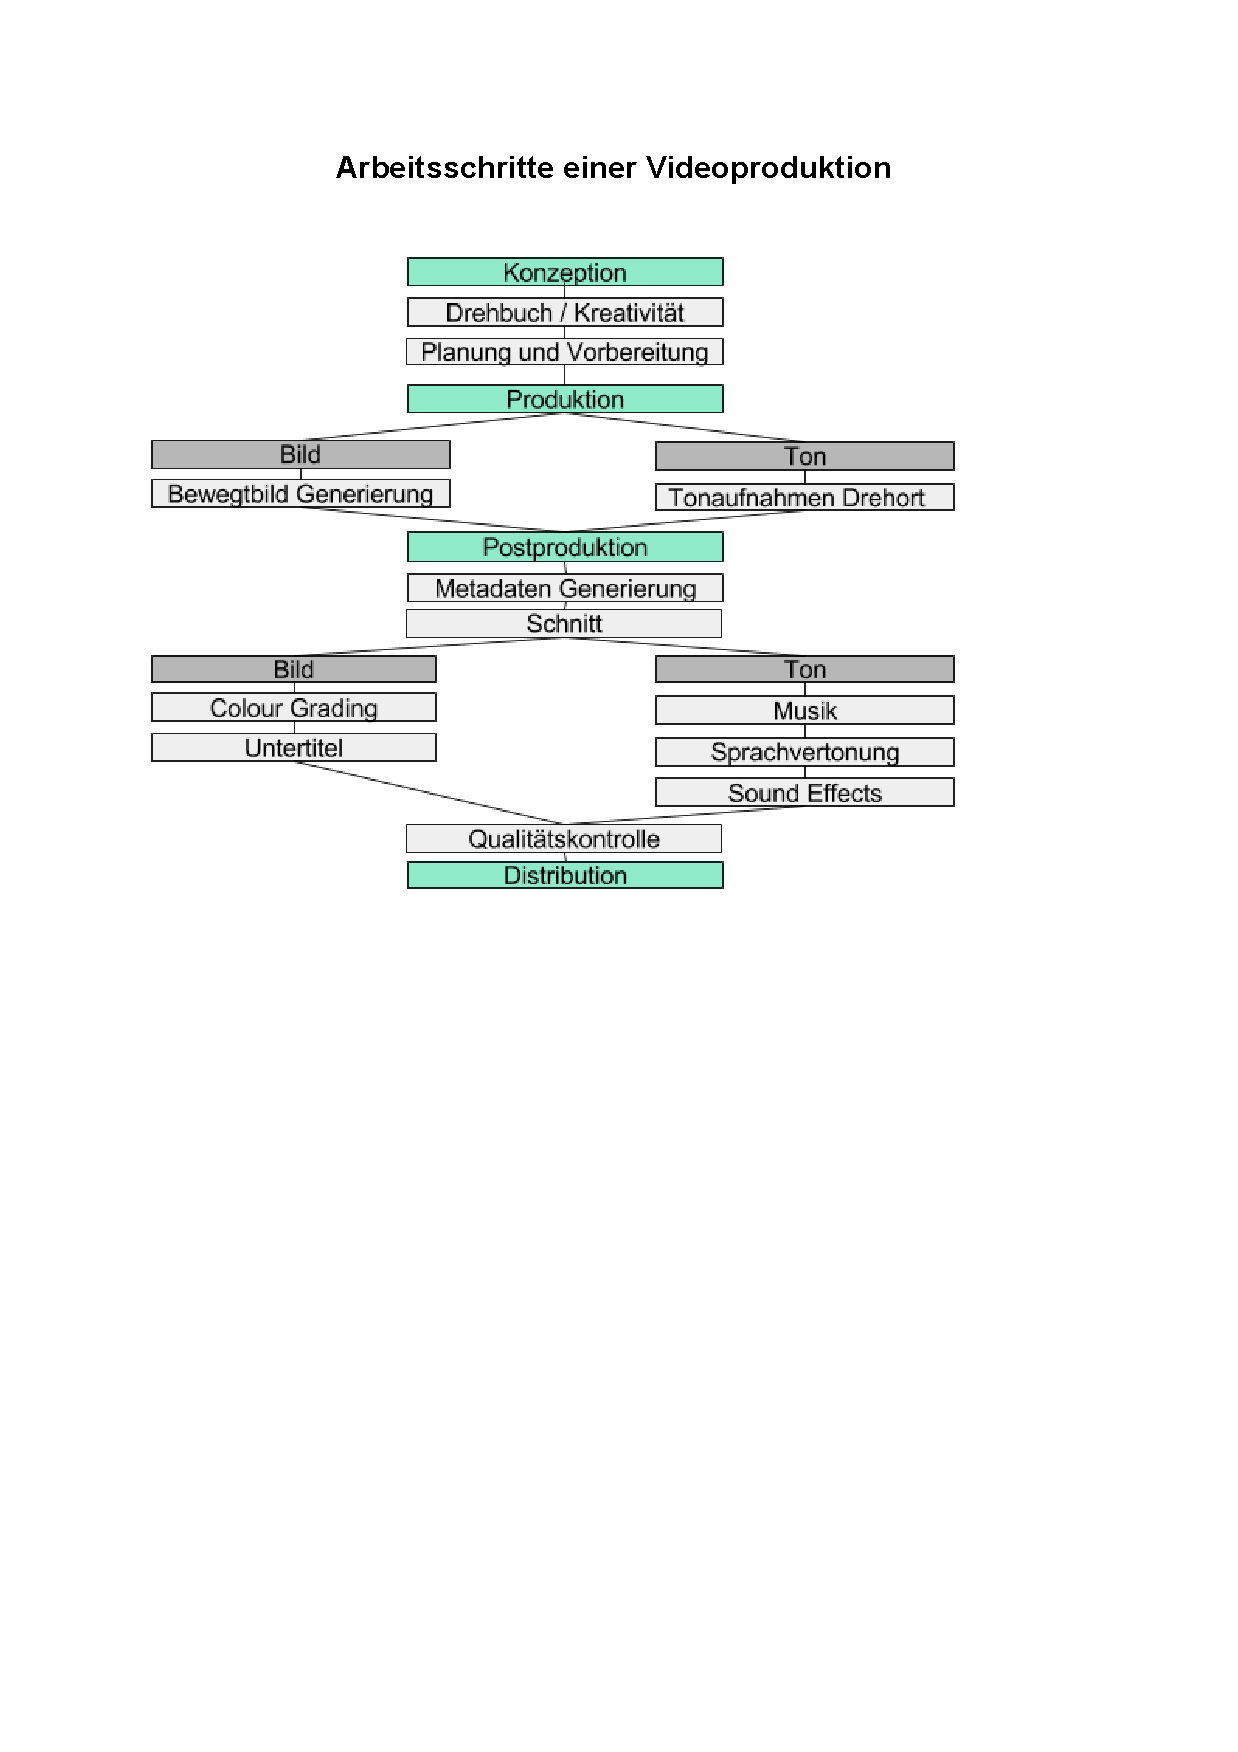
\includegraphics[width=\columnwidth, trim = 20mm 145mm 45mm 40mm, clip]{Bilder/ArbeitsschritteVideoproduktion.pdf}
	\caption{Grundlegende Arbeitsschritte einer Videoproduktion.}
	\label{fig:Videoproduktion}
\end{figure}
Mit der Bezeichnung Videoproduktion oder auch Filmproduktion wird die Herstellung von Kino-, Werbe- und Fernsehfilmen zusammengefasst. In Abbildung~\ref{fig:Videoproduktion} ist ein Ablaufplan einer typischen Videoproduktion zu sehen. Da es alleine in Deutschland über 850 Produktionsformen gibt (Stand 2014)~\cite{formatt}, kann der Ablaufplan nur einen sehr allgemeinen Überblick über die notwendigen Arbeitsschritte bieten. \\
Der erste Schritt, die Konzeption soll sowohl die Projektentwicklung, als auch die Vorproduktion zusammenfassen. Die sich anschließende Produktionsphase kann grob, wie im Schaubild zu dargestellt, in Bild und Ton unterteilt werden. Diese beiden Bereiche sollten nicht immer getrennt voneinander betrachtet werden. Die Postproduktion besteht aus vielen verschiedenen Arbeitsschritten, deren Schwerpunkt auf dem Schnitt und der digitalen Bildnachbearbeitung liegt. Der Schritt der Distribution ist hier der Vollständigkeit halber erwähnt und beschreibt die Filmverwertung. \\
Der Aufbau der folgenden Ausführungen orientiert sich an Abbildung~\ref{fig:Videoproduktion} (vgl. Kapitel~\ref{sec:Konzeption},~\ref{sec:Produktion} und~\ref{sec:Postroduktion}).



\SubSection{Neuronale Netze} \label{sec:NeuronaleNetze}
\todo[inline, color=yellow]{Laura} 
NN finden unter anderem Anwendung bei der Steuerung von Robotern, Börsenkursanalysen, Medizintechnik oder Fahrzeugsteuerung. In der Bildverarbeitung werden NN vor allem zur Klassifizierung genutzt. \\
Sie sind vom menschlichen Gehirn inspiriert, welches laut~\cite{NNHaykin} ein nicht-lineares, komplexes und hoch paralleles System zur Verarbeitung von Informationen darstellt. Ähnlich wie dieses bestehen künstliche NN aus einer Menge an simulierten Neuronen, die untereinander verbunden sind und in Schichten organisiert sind. Es gibt verschiedene Arten der Vernetzung, die, wie in \cite{NNHaykin} und \cite{NNStanley} beschrieben, in rück- und vorwärts gekoppelte Modelle unterteilt werden können.\\
\begin{figure}
	\flushleft
	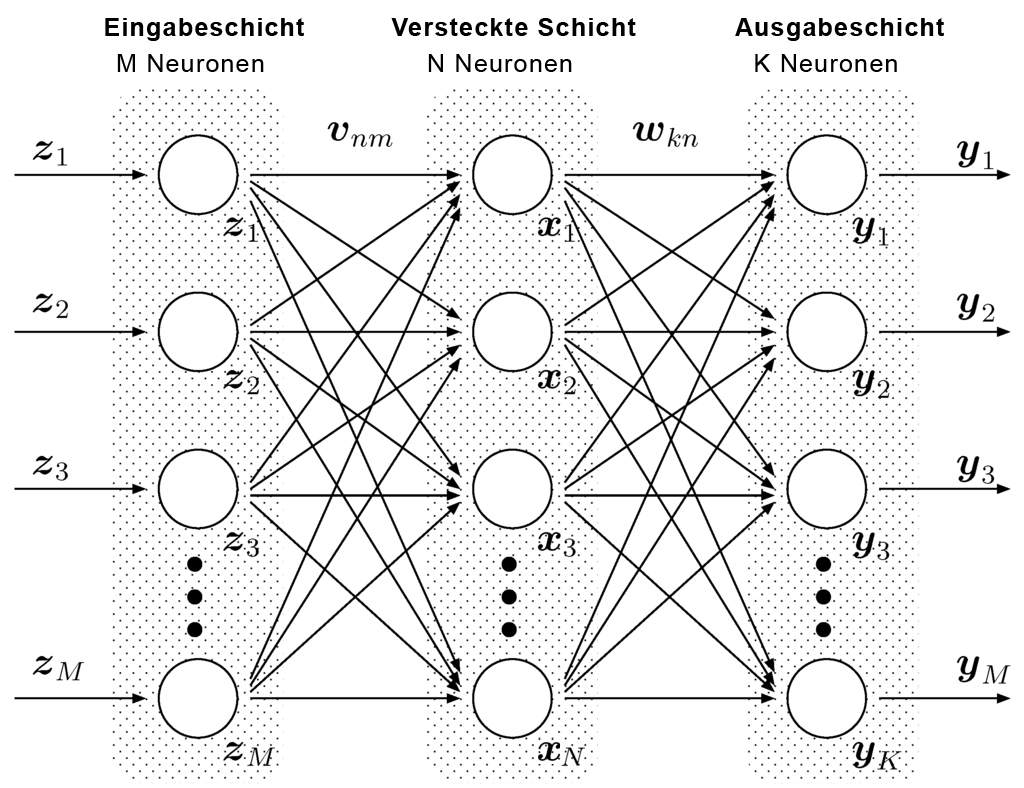
\includegraphics[width=\columnwidth]{Bilder/structure-mlp.jpg}
	\caption{Prinzipieller Aufbau MLP nach~\cite{MDPI}.}
	\label{fig:MLP}
\end{figure}
Am häufigsten kommen sogenannte \textit{Multilayer Perceptrons}~(MLP)~\cite{NNBraun}\cite{NNNauck}\cite{NNStanley} zum Einsatz, welche eine einfache Systemarchitektur haben. Der generalisierter Aufbau ist beispielhaft in Abbildung~\ref{fig:MLP} zu sehen. Dieses MLP besteht aus einer Eingabe- und Ausgabeschicht mit $M$ bzw. $K$ Neuronen und einer versteckten Schicht mit $N$ Neuronen. Es handelt sich um ein vorwärtsgekoppeltes Modell, bei welchem jedes Neuron einer Schicht mit jedem Neuron der darauffolgenden Schicht verbunden ist. Dies nennt man volle Verbindung. \\
Die Eingangsschicht dient zum Verteilen der Daten $z_m$ mit $m=1,...,M$. Die Ausgabe eines jeden Neurons in der versteckten Schicht, dargestellt durch $x_n$ mit $n=1,...,N$, lässt sich durch Formel~\ref{eq:AusgabeVerdeckteSchicht} berechnen. Hierbei steht $v_{nm}$ für die jeweilige Gewichtung der Verbindungen zwischen den Neuronen der Eingabe- und der versteckten Schicht und $f$ für die Aktivierungfunktion~\cite{NNStanley}\cite{NNHaykin} des jeweiligen Neurons. 
\footnotesize
\begin{equation} 
x_n = f~(\sum_{m=1}^M v_{nm}z_m)
	\label{eq:AusgabeVerdeckteSchicht}
\end{equation}
\small
Die Ausgangswerte $y_k$, mit $k=1,...,K$, lassen sich äquivalent unter Berücksichtigung der Werte $x_n$ und der Gewichte $w_{kn}$, sowie einer Aktivierungsfunktion $g$ berechnen, und gelten als Vertrauenswerte. Sie müssen gemäß der Aufgabenstellung interpretiert werden. 


\SubSection{Faltungsnetze} \label{sec:Faltungsnetze}
Im Folgenden wird detaillierter auf CNNs eingegangen, da diese die Grundlage für die meisten der hier vorgestellten Ansätze bilden. Vereinfacht ausgedrückt besteht ein CNN aus einer Vernetzung von Faltungsoperationen mit unterschiedlichen Filtermasken. CNNs kommen, bedingt durch ihre Architektur, oft zum Einsatz, wenn große Datenmengen von einem NN verarbeitet werden sollen. Ein schematischer Aufbau ist in Abbildung~\ref{fig:CNN} zu sehen. \\
\begin{figure}
	\flushleft
	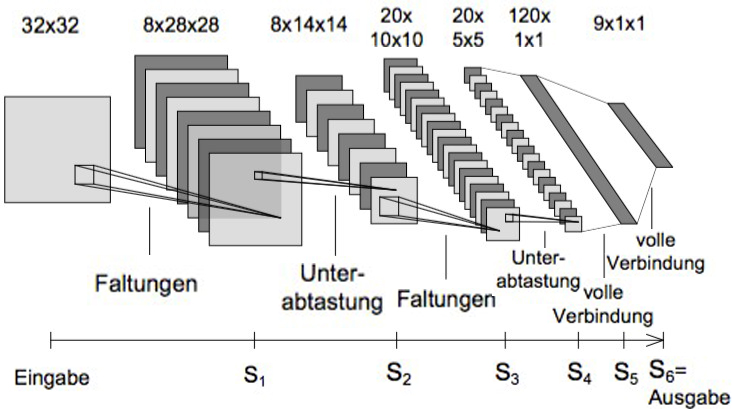
\includegraphics[width=\columnwidth]{Bilder/structure-cnn.jpg}
	\caption{Prinzipieller Aufbau Faltungsnetz nach~\cite{Osadchy}.}
	\label{fig:CNN}
\end{figure}
Jedes Pixel eines Feldes, das auf der Abbildung zu sehen ist, wird durch ein Neuron repräsentiert. Die Felder sind in Schichten organisiert. Die Eingangsschicht fungiert, vergleichbar mit den MLP aus Kapitel~\ref{sec:NeuronaleNetze}, als Verteiler der Information an die Neuronen der nächsten Schicht $S_1$. Die Besonderheit eines CNN sind die sich abwechselnd durchgeführte Faltung und anschließende Unterabtastung. Zwischen den Schichten $S_4$ und $S_6$ ähnelt das Modell einem MLP, da die Neuronen schichtweise voll verbunden sind.\\
Im Allgemeinen wird für eine Faltung eine Filtermaske $h$, also ein endlicher, zweidimensionaler Koeffizientensatz, wie in Formel~\ref{eq:Filtermaske} zu sehen, verwendet. Hierbei stehen $x$ und $y$ jeweils für die horizontale bzw. die senkrechte Bildkoordinate. Die Anzahl der Koeffizienten $a_{xy}$, wird in der Horizontalen mit $N_{hx}$ und im Vertikalen mit $N_{hy}$ bezeichnet.
\footnotesize
\begin{equation} 
	h(x,y) = \left\lbrace
  \begin{array}{l@{}l}
   0~f\ddot{u}r~x<-\lfloor\frac{N_{hx}-1}{2}\rfloor~\vee~y<-\lfloor\frac{N_{hy}-1}{2}\rfloor\\
    0~f\ddot{u}r~x>\lfloor\frac{N_{hx}-1}{2}\rfloor~~~~\vee~y>\lfloor\frac{N_{hy}-1}{2}\rfloor \\
    a_{xy}
  \end{array}
  \right.	
	\label{eq:Filtermaske}
\end{equation}
\small  
Formel~\ref{eq:Faltung} beschreibt die Faltung eines Eingangssignals $s$ mit einer Filtermaske $h$, wobei I das Ausgangssignal in Abhängigkeit von $x$ und $y$ beschreibt.
\footnotesize
\begin{equation}
\begin{aligned}
I(x,y) = (s*h)(x,y) = \\
\sum_{m_x=-\infty}^\infty \sum_{m_y=-\infty}^\infty s(m_x,m_y) \cdot h(x-m_x,y-m_y) 
\end{aligned}
	\label{eq:Faltung}
\end{equation}
\small
Im Fall eines CNN wird die Faltung, wie in Abbildung~\ref{fig:CNN}, beispielsweise zwischen der Eingangsschicht und $S_1$ vollzogen und durch die Verbindung zwischen den Neuronen zweier Felder modelliert. Dabei entsprechen die Gewichte der Neuronen genau den Filterkoeffizienten $a_{xy}$. Für ein jedes Feld sind diese Koeffizienten konstant, was bedeutet, dass alle Neuronen eines Feldes mit nur einem Gewicht auskommen. Dieses Prinzip nennt man geteilte Gewichte. \\
Im CNN wird nach jeder Faltung eine Unterabtastung durchgeführt um zu gewährleisten, dass die Dimension der Eingangsdaten schrittweise an die Dimension des Ausgangsvektors angepasst wird. Hierzu wird meist eine bilineare Unterabtastung um den Faktor 2 vorgenommen. Allgemeiner betrachtet werden $n$x$n$ Werte zu einem Wert zusammengefasst.\\
Wie zu Beginn des Kapitels erwähnt, haben CNNs gegenüber den MLPs den Vorteil, dass sie nahezu beliebig hochskaliert werden können und somit gut geeignet für große Datenmengen sind. Dies liegt vor allem daran, dass die Neuronen nur lokal verbunden sind und sich somit das Prinzip der geteilten Gewichte zu Nutze gemacht werden kann. Ein weiterer Vorteil von CNNs, der vor allem in der Bildverarbeitung genutzt wird, ist das sie translationsinvariant sind.

\SubSection{Training Faltungsnetze} \label{sec:Training}
Meistens werden CNN mittels der \textit{back-propagation} Methode trainiert. Bei dieser überwachten Lernmethode bedarf es einer großen Menge an vorab klassifizierten Trainingsdaten~\cite{5537907}.  \\
In den Faltungsschichten kann der Fehler der vorangegangen Schicht nach Formel \ref{eq:Training} berechnet werden. Dabei steht $E$ für den Fehler in der jeweiligen Schicht $l$ gemacht wird. Während $x^l$ für die Eingabe in die Schicht steht, bezeichnet $y^l$ die Ausgabe der entsprechenden Schicht. Die Größe der Eingabe wird der Einfachheit halber als quadratisch, also $mxm$-groß angenommen. Die Gewichtung wird mit $w$ bezeichnet. Um die Formel in der Realität anzuwenden, muss die linke und obere Grenze de Eingabeinhaltes, z.B. eines Bildes, mit Nullen ergänzt werden. Ansonsten wäre es nicht möglich den Fehler für Pixel zu berechnen, welche näher als $m$ an den entsprechenden Rändern liegen. \textcolor{red}{Ich würde das Delta gerne klein lassen, weil ich die Formel an zwei Stellen so gefunden habe :)}\\
\footnotesize
\begin{equation}
\begin{aligned}
\frac{\delta E}{\delta y_{ij}^{l-1}} = \sum_{a=0}^{m-1} \sum_{b=0}^{m-1} \frac{\delta E}{\delta x_{(i-a)(j-b)}^{l}} \frac{\delta x_{(i-a)(j-b)}^{l}}{\delta y_{ij}^{l-1}}  \\
= \sum \limits_{a=0}^{m-1} \sum \limits_{b=0}^{m-1} \frac{\delta E}{\delta x_{(i-a)(j-b)}^{l}} w_{ab}
\end{aligned}
	\label{eq:Training}
\end{equation}
\small
Die Schichten, in denen die Unterabtastung stattfindet, leisten kaum Beitrag zum eigentlichen Lernprozess des CNN. Hier wird das Problem allerdings reduziert, da $n$x$n$ Werte in einem einzigen resultieren. \\
Weil alle Gewichtungen $w$ mittels des \textit{back-propagation} Algorithmus während des Trainings angepasst werden, können CNN laut LeCun als Erzeuger ihrer eigenen Merkmalsextraktion gesehen werden \cite{LeCun:1998:CNI:303568.303704}.


\Section{Konzeption} \label{sec:Konzeption}
\todo[inline, color=yellow]{Vera} 
Vor der eigentlichen Produktion von Videomaterial muss das Projekt zunächst konzipiert und detailliert geplant werden. Dies bezieht sich vor allem auf die kreativen Prozesse des Drehbuchschreibens und die darauffolgende gesamte Projektplanung und -vorbereitung. Naturgemäß sind NN weniger sinnvoll für die Planung und das Management von Projekten. Doch in den letzten Jahren wurde versucht mit Hilfe von NN kreative Prozesse umzusetzen, wie sie für das Schreiben von Drehbüchern benötigt werden. Es gibt bereits erste Versuche mit Hilfe von NN automatisch sinnvolle Texte und Dialoge zu erstellen, die auf bekannten Texten und Storylines basieren \cite{Thoma16}. Dieses Verfahren wird in der Literatur auch \textit{Deep Writing} genannt. \textbf{Es können auch Romane, Dialoge oder Songtexte automatisch mit einem rückgekoppelten NN erstellt werden~\cite{DrehbuchWrite}.}

\SubSection{Aktueller Stand} \label{sec:SOTAVorverarbeitung}
\todo[inline, color=yellow]{Vera} 
\textbf{Ein solches rückgekoppeltes NN wurde mit allen bekannten Episoden der Serie \textit{Silicon Valley} trainiert \cite{DrehbuchSV}}. Zu Beginn des Schreibprozesses wird ein beliebiges Wort genutzt um den ersten Satz zu initialisieren. Das NN sucht im Anschluss das Wort, welches am häufigsten nach dem Startwort in den Trainingsdaten genannt wurde. Mit diesem Wortpaar wird nach dem selben Prinzip das dritte Wort des Textes ermittelt. Dieser Prozess wird solange wiederholt bis der generierte Text die gewünschte Länge erreicht hat \cite{DrehbuchWrite}. Die generierten  grammatikalisch korrekten Sätze beziehungsweise Dialoge ergeben keine sinnvollen Zusammenhänge und folgen keiner ersichtlichen Storyline. Der Film \textit{Sunspring}~\cite{DrehbuchMovie} wurde nach einem ähnlichen Prinzip erstellt und im Anschluss von einem professionellen Filmteam realisiert. Der größte Unterschied zu \cite{DrehbuchSV} ist, dass das NN nicht nur Wörter unterscheidet. Stattdessen wird zunächst alles in Buchstaben zerlegt und dann in neue Wörter und Sätze zusammengesetzt. Das verwendete NN nannte sich selber \textit{Benjamin} und wurde mit einer großen Anzahl an Drehbüchern von Science Fiction Filmen aus den 80er und 90er Jahren trainiert. \textbf{Heraus kam ein Drehbuch, welches qualitativ  mit den Resultaten des ersten Ansatz vergleichbar ist. Ein auffälliges Problem war der korrekte Umgang mit Namen, da diese sprachlich anders behandelt werden. Aus diesem Grund konnten alle Charaktere nur mit einem Buchstaben benannt werden. Dies hatte zur Folge, dass das NN zwei Charaktere gleich benannt hat und sie nachträglich manuell umbenannt werden mussten.}\\

\textbf{Selbst mit einer sehr großen Anzahl von Trainingsdaten konnten keine kohärenten Dialoge generiert werden und keine konstante und neue Storyline verfolgt werden.  Daraus lässt sich ableiten, dass zum jetzigen Zeitpunkt NN große Schwierigkeiten haben neue Ideen zu entwickeln und Erlerntes innerhalb größerer Zusammenhänge sinnvoll zu verknüpfen. Deshalb kann derzeit der Aufwand des Drehbuchschreibens durch NN nicht reduziert werden.}

\Section{Produktion} \label{sec:Produktion}
Die Produktion ist von allen drei besprochenen Kategorien diejenige, die bisher am wenigsten automatisiert durchgeführt werden kann. Moderne Kameras- und Tonaufnahmesysteme bieten zwar eine einfachere Handhabung und Fehlerkontrolle, als es noch bei der analogen Aufzeichnung der Fall war, dennoch braucht eine Filmproduktion viele menschliche Arbeitsstunden. \\
Im Folgenden soll geprüft werden, ob es heutzutage realisierbare Automatiersungsansätze gibt. Dabei wird oberflächlich auf die Generierung von Musik eingegangen, die später in der Postproduktion unter die einzelnen Szenen gelegt werden kann. Daran schließt sich eine ausführlichere Betrachtung eines Ansatzes zur automatisierten Generierung von Szenen Dynamiken an. 


\SubSection{Aktueller Stand Musikgenerierung} \label{sec:SOTAProduktion}
Es gibt verschiedene Ansätze NN zu nutzen, um Musik automatisiert generieren zu lassen. Im Folgenden werden drei Ansätze kurz vorgestellt, welche alle rückgekoppelte Neuronale Netze (RNN) benutzen. \\
An der \textit{University of Washington} ist im Rahmen einer Projektarbeit ein Musik Generator namens \textit{Algo Rythm} entstanden~\cite{Algorithm}. Für die Umsetzung haben die Studierenden um \textit{Timmerman} mehrere RNN geeignet trainiert. Der Quellcode kann auf \textit{Github} \cite{AlgorithmGit} eingesehen werden.\\
Ein weiterer Ansatz, der in~\cite{eck+lapalme:2008} beschrieben wird, arbeitet ebenfalls mit einem RNN, welches mit einem Autokorrelation-basierten Prädiktor \textcolor{red}{Prädiktor = "Vorhersager" denke das Wort kennt der Reiter die p-Bilder bei ner GOP sind ja auch prädiktiv} kombiniert wird. Dabei soll die Struktur von Musikstücken erlernt werden, indem zunächst die folgende Note einer Tonreihenfolge vorausgesagt wird. \\
Der letzte Ansatz benutzt ebenfalls RNN um auf Grundlage einer Notensequenz eine Musikstück zu komponieren~\cite{browne2001system}. Dabei wird die Eingabesequenz zunächst interpretiert. Anschließend sorgen zwei RNN-basierte Algorithmen für die Produktion von sowohl Rhythmus, als auch die Vorhersage der nächsten Note. \\

Alle drei Ansätze weisen hohes Potential auf, wenn es darum geht Musikstücke automatisch zu generieren. Über das Genre des zugeführten Musikmaterials lässt sich die gewünschte Ausgabe begrenzt steuern. Es wäre durchaus vorstellbar, diese automatisch generierte Musik für eine Filmproduktion zu benutzen.
\textcolor{green}{Memo an mich selber: Hier evtl. mehr schreiben}


\SubSection{Generierung von Videos mit Szenen Dynamiken} \label{sec:Vondrick}
Mit dem Ansatz von Vondrick et al.~\cite{VondrickPT16} können aus Einzelbildern ganze Szenen Dynamiken erstellt werden, welche für die Klassifizierung oder für die Vorhersage von Bewegungen genutzt werden können. Das Resultat sind kleine Bildsequenzen mit einer Auflösung von 64x64 Pixeln und 32 Einzelbildern. \\
Die Grundlage für dieses Verfahren bilden zwei CNN, die als \textit{Generative Adversarial Networks} (GAN) \cite{NIPS2014_5423} fungieren. \textcolor{green}{Memo an mich selber: Hier evtl. mehr schreiben}Beide Netze können als Gegenspieler angesehen werden. Während der Generator $G$ für die Generierung von einer Videosequenz auf Grundlage eines Standbildes zuständig ist, soll der Diskriminator $D$ zwischen den so erzeugten und realen Videosequenzen differenzieren können. Um dies zu erreichen werden beide GAN, wie in Formel 1 des Papers~\cite{VondrickPT16} zu sehen gegeneinander trainiert. Das Minimierungs- bzw. Maximierungsproblem wird hierzu mittels Gradientenverfahren gelöst. \\
Das Training der beiden Netze erfolgt unüberwacht. Da ähnliche Objekte in der Regel auch ähnliche Bewegungsmuster aufweisen, lassen die Autoren das zur Verfügung stehende Videomaterial in Kategorien (Strand, Babys, Golf und Züge) einteilen. Zudem sorgt ein Stabilisierungsalgorithmus dafür, dass bei dem gesamten Testmaterial von einer statischen Kamera ausgegangen werden kann und die zu erlernende Szenen Dynamik nicht durch eine Bewegung der Kamera verfälscht wird. Für jede dieser Kategorien wird dann ein eigenes Pärchen bestehend aus Generator und Diskriminator trainiert. \\
Bevor die beiden CNN $G$ und $D$ auf die beschriebene Art trainiert werden können, müssen sie erst einmal ihren Aufgaben entsprechend aufgebaut werden. \\
\begin{figure}
	\flushleft
	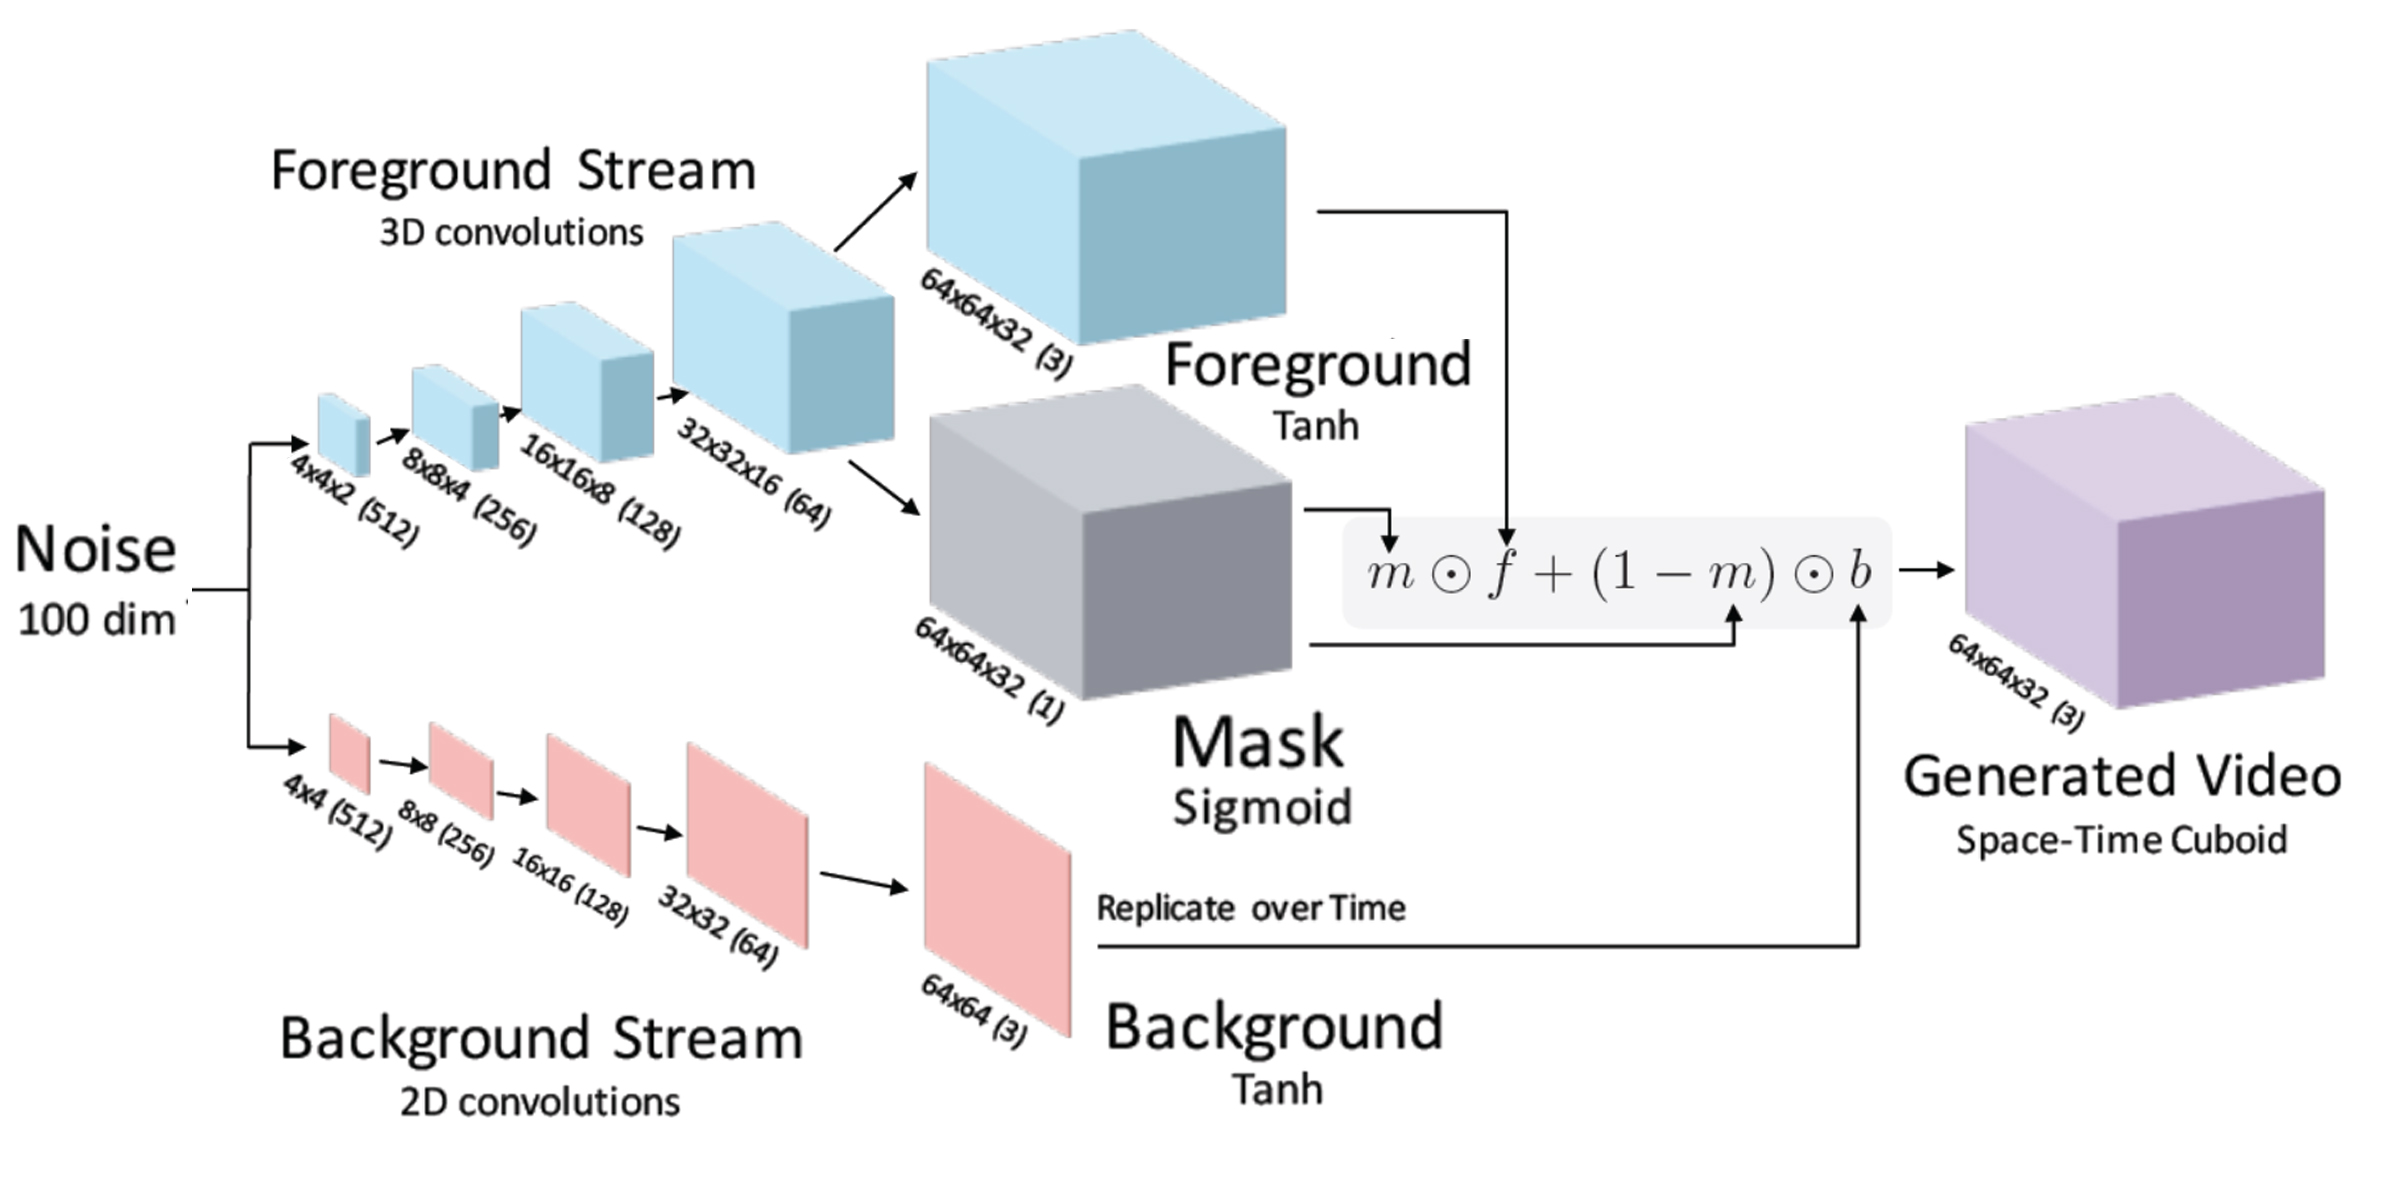
\includegraphics[width=\columnwidth]{Bilder/generator2.jpg}
	\caption{Aufbau Generator nach~\cite{VondrickPT16}.}
	\label{fig:generator}
\end{figure}
Den Aufbau des genutzten Generators \cite{VondrickPT16} ist in Abbildung~\ref{fig:generator} zu sehen. Im Gegensatz zu dem in Kapitel~\ref{sec:Faltungsnetze} beschriebenen, gewöhnlichen CNN, wird hierbei keine Unterabtastung vorgenommen, sondern die Menge der Daten von Schicht zu Schicht erweitert. Zudem werden die Eingabedaten für die Verarbeitung in zwei Datenströme aufgeteilt. Während in dem einen Strom der statische Hintergrund entsprechend vergrößert wird, wird in dem anderen die Bewegung des sich im Vordergrund befindlichen Objektes vorhergesagt. Beide Teile werden dann am Ausgang nach Formel~\ref{eq:Generator} zusammengefasst.
\footnotesize
\begin{equation}
\begin{aligned}
G(z) = m(z) \odot f(z) + (1-m(z))\odot b(z)
\end{aligned}
	\label{eq:Generator}
\end{equation}
\small
Dafür ist die binäre Maske $m$ so gewählt, dass sie überall den Wert eins hat, wo der Vordergrund übernommen werden soll und ansonsten nur Nullen enthält. \\
Der Diskriminator hat eine typische Faltungsnetzarchitektur, die in Abbildung~\ref{fig:discriminator} zu sehen ist. Dabei muss seine Eingabeschicht eben so groß sein, wie die Ausgabeschicht des Generators.\\
\begin{figure}
	\flushleft
	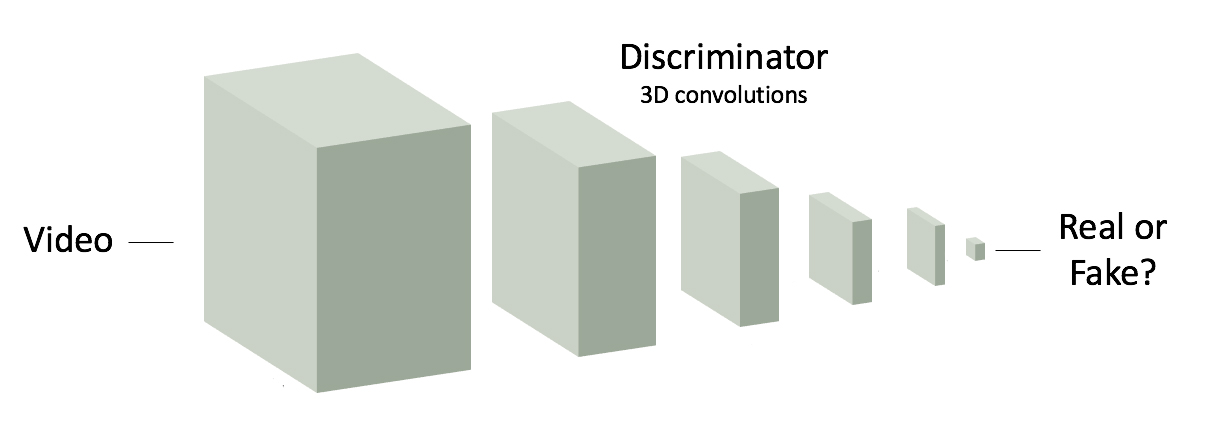
\includegraphics[width=\columnwidth]{Bilder/discriminator.jpg}
	\caption{Aufbau Diskriminator nach~\cite{VondrickPT16}.}
	\label{fig:discriminator}
\end{figure}
Die Bedeutung für so erzeugte Bewegtbildsequenzen für die Automatisierung der Produktion von Filmen, wird im nächsten Kapitel diskutiert. Die Resultate können auf der Internetseite der Autoren eingesehen werden~\cite{VondrickInternet}.


\textcolor{green}{Memo an mich selber: Das gesamte Kapitel noch einmal überdenken}



\SubSection{Bewertung des Ansatzes von Vondrick} \label{sec:VondrickConclusion}
Das in Kapitel~\ref{sec:Vondrick} beschriebene Verfahren schafft es automatisiert aus einem Einzelbild eine kurze und niedrig aufgelöste Bewegtbildsequenz zu erstellen. Hierbei wird vor allem die Szenen Dynamik in den meisten Fällen annähernd realistisch vorhergesagt, wobei die Modellierung des sich bewegenden Bildinhaltes eher mangelhaft ist. Trotz des hohen Bedarfs an Trainingsmaterial und den damit verbundenen Zeitaufwand, kann das System ohne menschliche Hilfe eigenständig Kategorisieren, Trainieren und letztendlich Szenen Dynamiken generieren. Gegen einen Einsatz in der Videoproduktion sprechen die geringe Auflösung und Zeitspanne die bisher generiert werden kann. Zudem kann in einer Szene nicht immer nur von einem sich bewegenden Objekt ausgegangen werden. Weiter ist das Training der Netzen für alle denkbaren Kategorien sehr aufwendig. Dennoch könnte der Ansatz als Grundlage für einen ausgereifteren Algorithmus dienen, der beispielsweise die Anweisungen des Drehbuchs mit einbezieht und somit bessere Orientierung entlang der Storyline gewährleitest. \textcolor{red}{Kann man das so schreiben??}\\
Der jetzige Stand des Algorithmus könnte beispielsweise für die Generierung von GIFs oder Simulationen genutzt werden. Zudem könnte der Ansatz, mit etwas Anpassung, anstatt Szenen Dynamiken in Form von Videos darzustellen, Bewegungsvektoren aus einem Standbild vorhersagen und somit in der Videocodierung Einsatz finden. \textcolor{green}{Memo an mich selber: Das gesamte Kapitel noch einmal überdenken; Veras Vorschlag: Zudem könnte der Ansatz nach einer geeigneten Anpassung Bewegungsvektoren aus einem Standbild vorhersagen, welche in der Videocodierung Einsatz finden.}




\Section{Postproduktion} \label{sec:Postroduktion}
\todo[inline, color=yellow]{Vera} 
\textbf{In diesem Kapitel wird die Verwendung von NN in der Postproduktion beschrieben. Gerade in diesem Produktionsabschnitt finden NN eine breites Anwendungsfeld, da die CNN im Bereich der Bildverarbeitung in den letzten Jahre sehr erfolgreich eingesetzt werden konnten. Im ersten Abschnitt werden zunächst die interessantesten auf NN-basierenden Ansätze für Postproduktion vorgestellt und bewertet. Im Anschluss werden zwei Verfahren zur Stilsynthese detailliert beschrieben und für den Einsatz in der professionellen Videoproduktion analysiert. Zuletzt wird ein Ausblick auf Einsatzmöglichkeiten gegeben. }

\SubSection{Aktueller Stand} \label{sec:SOTAPostproduktion}
\todo[inline, color=yellow]{Vera} 
\textbf{Für einige Produktionen, wie Dokumentationen oder Nachrichtensendungen, werden \textit{Voice-Over} benötigt.\textbf{ Teilweise werden diese bereits mit sogenannten \textit{Text-to-Speech}- Verfahren produziert, doch die Stimmen klingen meist sehr künstlich. }\\
Ein vielversprechender Ansatz ist \textit{WaveNet}, welcher im Gegensatz zu den meisten anderen NN-basierten Ansätzen ein CNN verwendet. Dieses wird mit Text- und Audiodatenpaaren von realen Sprechern trainiert und die künstlich erzeugten Stimmen klingen sehr natürlich und menschlich~\cite{OordDZSVGKSK16}.} Das \textit{Deep Voice} Verfahren~\cite{DeepVoice} entwickelt das \textit{WaveNet} Verfahren weiter. Während \textit{WaveNet} mehrere Minuten Rechenzeit benötigt um eine Sekunde an Audiodaten zu generieren, ist \textit{Deep Voice} Realtime-fähig und ein eigenständiges System. Dadurch ist es für die Nutzung in der Videoproduktion interessanter. Einen Vergleich bezüglich der Klangqualitätsunterschiede zwischen den beiden Verfahren gibt es in der Literatur leider nicht.
\\
Nachdem alle notwendigen Daten produziert wurden sollten diese gekennzeichnet und in eine entsprechende Mediendatenbanken eingepflegt werden. Die Kennzeichnung der Daten kann mit Hilfe von NN zuverlässig automatisiert werden, da in der Objektklassifikation mit CNN in den letzten Jahren eine sehr geringe Fehlerquote und hohe Robustheit erreicht werden konnte. Eine bekannte Bibliothek ist \textit{Clarifai}~\cite{MITReview}, welche konfigurierte CNN anbietet um optimierte Bild- oder Videodatenbanken anzulegen und zu verwalten.  Weitere aktuelle Veröffentlichungen~\cite{Ng_VideoLabelling}\cite{Ye:VideoLabelling}\cite{KangEABZ17} konzentrieren sich auf die Verbesserung der Leistungsfähigkeit um auch große Datenmengen robust zu kennzeichnen. Dies ist für die große Menge an Videodaten einer Filmproduktion ein wichtiges Kriterium. Zum jetzigen Zeitpunkt erfordert die Erkennung dieser Mengen noch sehr große Rechenkapazitäten und ist entsprechend kostenintensiv. \\

\textbf{Neben der verbreiteten Klassifikation können CNN auch Bilddaten generieren und den Stil eines Bildes übertragen. Zwei vielversprechende Stilsynthese-Ansätze sind das \textit{Deep Dream}~\cite{DeepDream} und das \textit{Deep Style} Verfahren~\cite{GatysEB15a}. Im Gegensatz zu anderen bekannten Verfahren können diese CNN-basierten Verfahren die gesamte Bildsemantik eindeutig vom Inhalt trennen und mit einem anderen Bildes verschmelzen ohne dessen Inhalt zu verändern~\cite{McCaigDG16}. Diese beiden Verfahren werden in den nächsten Abschnitten genauer beschrieben.}

\SubSection{Faltungsnetze zur Stilsynthese}\label{sec:Stilsynthese}
\todo[inline, color=yellow]{Vera} 
Das Verständnis der folgenden Algorithmen in Abschnitt~\ref{sec:DeepDream} und~\ref{sec:DeepStyle} setzt ein grundlegendes Verständnis der Prozesse innerhalb eines CNN voraus. In Abbildung~\ref{fig:CNN} wird deutlich, dass mit jeder Schicht das Bild stärker unterabgetastet wird und die Größe der Merkmalsvektoren stetig steigt. Mit jeder weiteren Schicht wird ein größer Ausschnitt des Bildes erfasst und dessen Merkmale extrahiert. Die Merkmalsvektoren werden größer, da ein größerer Bereich mehr Merkmale enthält und diese folglich immer komplexere Merkmale enthalten. \\
Im oberen Bereich der Abbildung~\ref{fig:StyleRepresenation} wird veranschaulicht, dass die stilgebenden Merkmale immer mehr der Semantik des Stilbildes annähern. Während in der ersten Schicht die Stilmerkmale sehr klein sind, können in den höherwertigen Schichten Stilelemente aus dem gesamten Bild gefunden werden, wie zum Beispiel die gelben Kreise und die Strudel im Himmel. Im untereren Abbildungsbereich sind die inhaltsbezogenen Merkmale dargestellt. Hier ist die Unterabtastung klar zu erkennen, doch das Gebäude bleibt stets identifizierbar. Die Inhaltsinformationen bleiben trotz der Unterabtastung erhalten.

Für ein besseres Verständnis der verborgenen Schichten wurde der Prozess zur Objekterkennung invertiert. Das trainierte CNN wurde mit einem Eingangsbild initialisiert, welches ausschließlich zufälliges Rauschen enthält. Dieses Eingangsbild wurde iteriert bis ein Objekt klassifiziert werden konnte. In diesem Bild konnten teilweise eindeutige Merkmale dieses Zielobjektes ausgemacht werden. An dieser Stelle sei hinzugefügt, dass das CNN ein Objekt nicht immer präzise bestimmen kann, da die Klassifikation stark von den Trainingsdaten abhängt. Zum Beispiel bei der Bestimmung von Hanteln kann es dazu kommen, dass auch Arme zum Merkmalsvektor hinzugefügt werden, da diese überdurchschnittlich häufig auf den Trainingsdaten mit den Hanteln zu sehen waren. 
Trotzdem lässt sich eindeutig nachweisen, dass CNN auch für die Generierung von Bilddaten genutzt werden und nicht ausschließlich für die Klassifizierung \cite{DeepDream}\cite{MahendranV14}.

Ein anderer Ansatz zur Analyse von CNN lässt es selbst entscheiden, welche Merkmale verstärkt werden. Ein beliebiges Eingangsbild wird durch das CNN propagiert und die Merkmalsvektoren der einzelnen Schichten untersucht. In den niedrigeren Schichten können nur primitive Texturmerkmale ausgemacht werden, wie Linien oder Rechtecke, während der Bildinhalt unverändert bleibt. Mit steigender Schichtanzahl werden die verstärkten Muster immer komplexer und größer während der Bildinhalt teilweise modifiziert wird. So wird deutlich, dass CNN in den höheren Schichten die benötigten Informationen der Semantik enthalten und diese eindeutig vom Bildinhalt separiert.\\
\begin{figure}
	\flushleft
	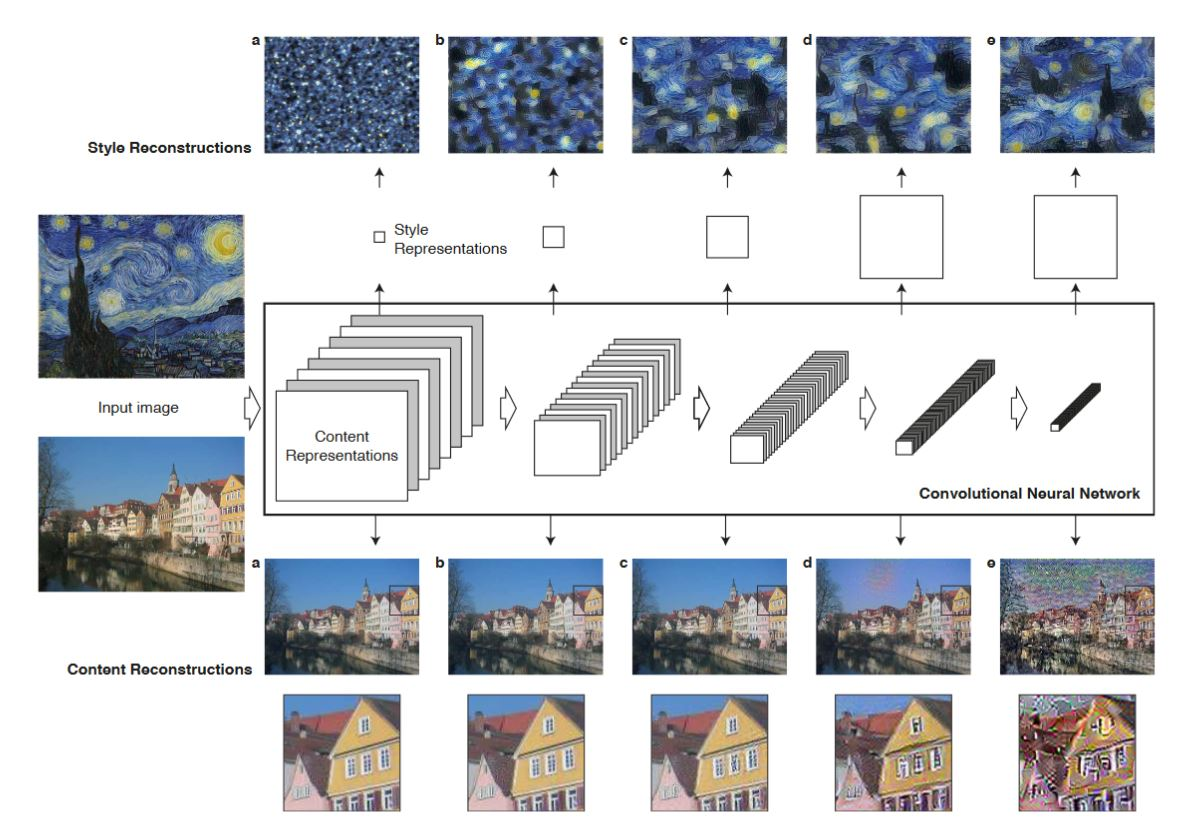
\includegraphics[width=\columnwidth]{Bilder/StyleRepesentation.JPG}
	\caption{Merkmalsextrahierung in einem Faltungsnetz\cite{GatysEB15a}.}
	\label{fig:StyleRepresenation}
\end{figure}

\SubSection{Deep Dream} \label{sec:DeepDream}
\todo[inline, color=yellow]{Vera} 
Der folgende Abschnitt stellt das Stilsynthese-Verfahren \textit{Deep Dream} \cite{DeepDream} vor, welches ein Nebenprodukt des Versuches den Inhalt eines CNN zu visualisieren ist. \textit{Deep Dream} basiert auf einem \textit{GoogLeNet} CNN mit 22 Schichten und fünf Unterabtastungsschichten~\cite{Szegedy_2015_CVPR}. Die Schichten haben eine besondere Architektur, welche \textit{Inception Layer} genannt wird. Mit Hilfe dieser Architektur können auch große Merkmalsvektoren effizient verarbeitet werden. Dieses \textit{GoogLeNet} wird im ersten Schritt mit dem \textit{\textit{ImageNet}}~\cite{ImageNet} Trainingsdatenset trainiert.\\
An dieser Stelle sei zum besseren Verständnis hinzugefügt, dass ein wichtiger Unterschied zu den bereits bekannten Faltungsnetzmodellen aus Abschnitt~\ref{sec:Faltungsnetze} besteht. Die Schichten zur Klassifizierung sind für die Stilsynthese nicht weiter relevant. Nur die Faltungsschichten werden verwendet, welche die benötigten Merkmalsvektoren extrahieren und speichern.\\
Zunächst wird das stilgebende Bild, im folgenden Style Source (SS) genannt, bis zu einer beliebigen Faltungsschicht vorwärtspropagiert und der entsprechende Merkmalsvektor als $\vv{f_{GS}}$ gespeichert. Dieser enthält die Merkmale der gewünschten Semantik und steuert die Transformation in Richtung des gewünschten Stils. Würde $\vv{f_{GS}}$ entfallen nähert das CNN die Transformation an die Trainingsdaten an.  Bezogen auf Abschnitt~\ref{sec:Stilsynthese} empfiehlt es sich höhere Schichten zu wählen um eine zufriedenstellendes Synthese zu generieren.\\
\begin{figure}
	\flushleft
	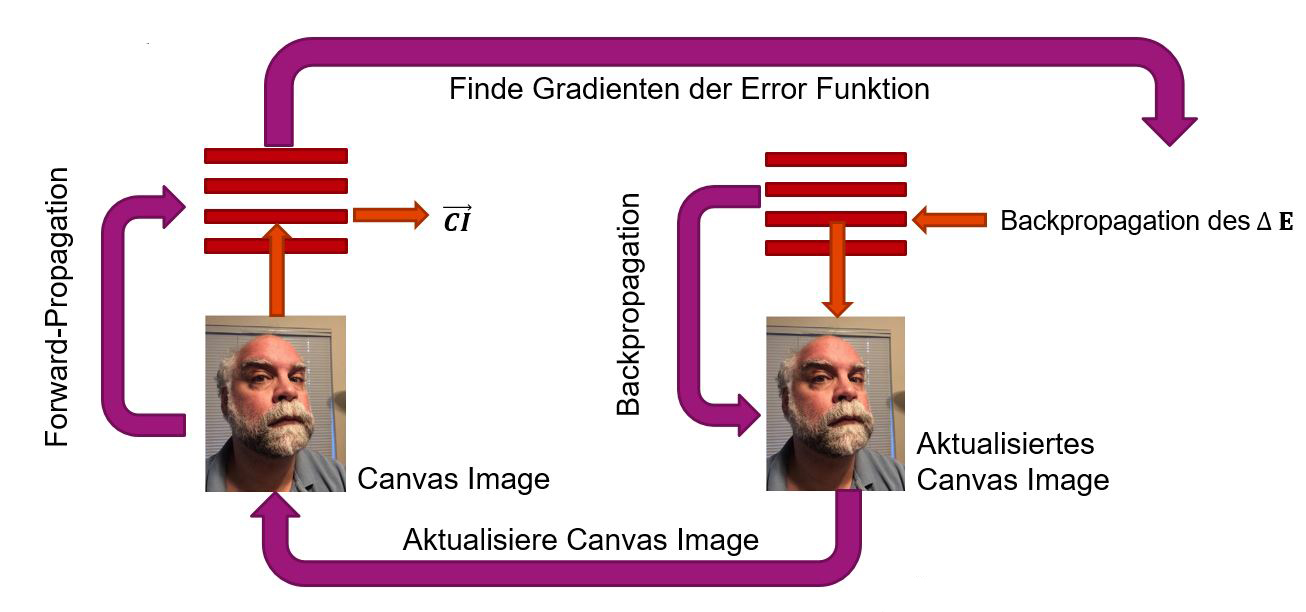
\includegraphics[width=\columnwidth]{Bilder/DeepDream.jpg}
	\caption{Ablaufdiagramm des Deep Dream Verfahrens.}
	\label{fig:DeepDream}
\end{figure}
Den weiteren Transformationsprozesses stellt Abbildung~\ref{fig:DeepDream} schematisch dar. Das Zielbild, im folgenden Canvas Image (CI) genannt, wird iterativ transformiert. Zu Beginn einer Iteration wird es bis zur selben Schicht wie $\vv{f_{GS}}$ vorwärtspropagiert und als $\vv{f_{CS}}$ gespeichert. Im Anschluss wird der Gradient der Fehlerfunktion $\Delta E(x,y)$ aus Gleichung~\ref{eq:DeepDreamError} berechnet. Der Fehler $\Delta E(x,y)$ wird demnach maximal, wenn die beiden Vektoren in die selbe Richtung zeigen.
\footnotesize
\begin{equation}
E(x,y)= \vv{f_{GS}}* \vv{f_{CS}}
\label{eq:DeepDreamError}
\end{equation}
\small
Der resultierende  $\Delta E(x,y)$ wird zurückpropagiert und die Gewichtungen innerhalb des Netzes in Richtung des SS korrigiert. Das daraus entstehende Bild wird als neues CI aktualisiert und für die nächste Iteration wiederverwendet.
Dieser Ablauf terminiert, wenn der Fehler minimal ist und $\vv{f_{CS}}$  möglichst weit dem Ausgangsbild $\vv{f_{GS}}$ angenähert ist. In diesem Fall ist $E(x,y)$ maximal und der gesamte Prozess wird als Maximierung von Gleichung~\ref{eq:DeepDreamError} interpretiert.\\

\begin{figure}
	\flushleft
	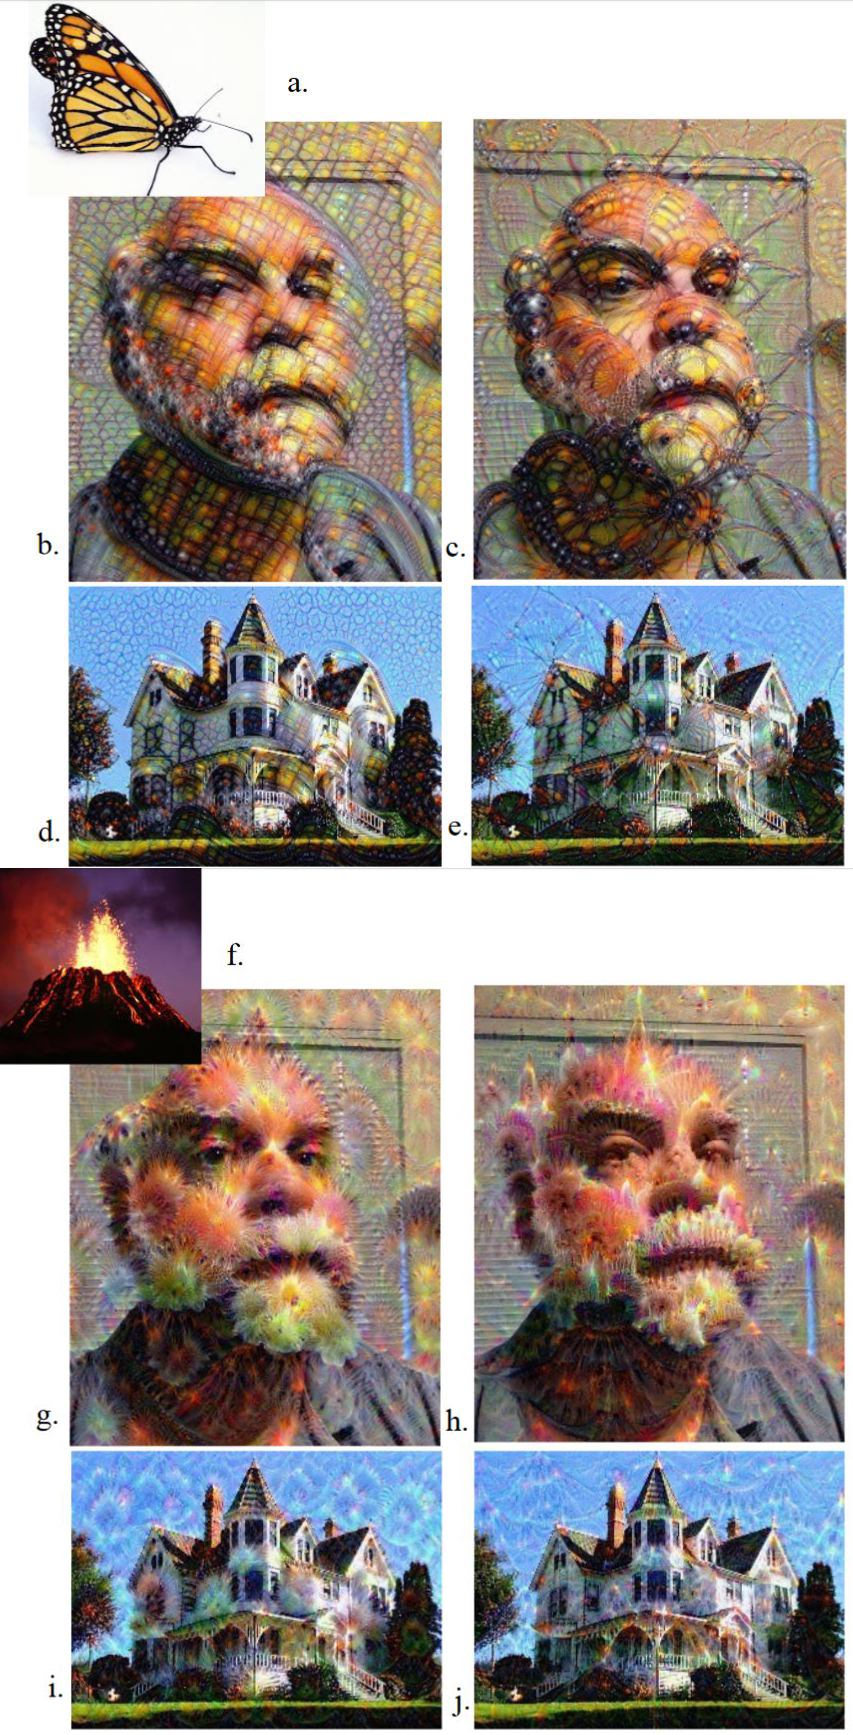
\includegraphics[width=\columnwidth]{Bilder/DeepDreamResults.JPG}
	\caption{Resultate des Deep Dream Verfahrens~\cite{McCaigDG16}.}
	\label{fig:DeepDreamResults}
\end{figure}

Einige Ergebnisse des \textit{Deep Dream} Verfahrens sind in Abbildung~\ref{fig:DeepDreamResults} dargestellt. Die kleinen Bilder in der oberen Ecke sind die verwendeten SS. Auf der linken Seite eines Blockes sind jeweils die Ergebnisse mit einer niedrigen Schicht und rechts die einer höheren Schicht dargestellt. Auf den ersten Blick fällt direkt auf das die linken Bilder stärker kleinere Merkmale skalieren und übernehmen. Rechts werden eindeutig größere Texturen berücksichtigt, wie zum Beispiel die Form des Schmetterlings oder Vulkans am Hals. Gleichzeitig fällt rechts auf, dass markante Bildpunkte, wie die Augen oder die Nase, in der Form modifiziert wurden. Somit gehen teilweise Inhalte des ursprünglichen Bildes verloren. Die Nase wurde teilweise einer Hundeschnauze angenähert, da die Trainingsdaten von \textit{ImageNet}~\cite{ImageNet} einen Überschuss an Hundemotiven enthalten. Besonders deutlich wird diese Tendenz, wenn kein SS verwendet wird~\cite{McCaigDG16}. Andere Ergebnisse zeigten auch deutlich, dass durchaus auch die Merkmale der Trainingsdaten gegenüber denen des SS überwiegen können.
\\
Es ist demzufolge für den Nutzer nicht möglich die Endergebnisse zu beeinflussen. Die einzige Möglichkeit der Kontrolle bietet die Wahl des SS und der Trainingsdaten, welche einen nicht vorhersehbaren Einfluss auf das Endergebnis haben. Daher kann von keiner strikten Trennung von Semantik und Inhalt ausgegangen werden. \\
Weiter kann nicht gewährleistet werden die Ergebnisse zu reproduzieren und ähnliche Bilder auf kohärente Weise zu transformierten, da die Gewichte des CNN stetig während einer Iteration modifiziert werden. Diese Reproduzierbarkeit und Kohärenz ist ein wichtiges Kriterium für die Videoproduktion, da eine Sequenz von ähnlichen Bilder entsprechen gleichförmig transformiert werden muss. Aus diesem Grund ist dieses Verfahren mehr eine neue Kunstform und interessante Weise die Funktionalität von CNN besser zu verstehen. Für die Videoproduktion ist sie gänzlich ungeeignet.



\SubSection{Deep Style}\label{sec:DeepStyle}
\todo[inline, color=red]{Vera} 
Gerade die mangelnde Einflussnahme und die fehlende Reproduzierbarkeit des Nutzers beim \textit{Deep Dream} Verfahren \cite{DeepDream} verlangt nach einer Weiterentwicklung. Diese ist durch das \textit{Deep Style} Verfahren \cite{GatysEB15a} gegeben, welche ein ähnliches Schema verfolgt. Der große Unterschied ist die strikte Trennung und Berücksichtigung von stilgebenden und inhaltsbezogen Informationen, einer erweiterten Fehlerfunktion und der Initialisierung durch ein Bild mit zufälligem Rauschen.\\
Zusätzlich wird eine andere CNN-Architektur verwendet. Es wird ein trainiertes CNN verwendet, dessen Architektur von der \textit{Visual Geometry Group} entwickelt wurde~\cite{SimonyanZ14a}. Es besteht aus 16-19 Schichten, welche in erster Linie aus $3\times3$ Faltungskernen besteht. Dieses CNN wurde ebenfalls mit dem \textit{ImageNet} Trainingsdatenset~\cite{ImageNet} trainiert.

Nach dem Training wird zunächst ein SS bis zur letzten Faltungsschicht vorwärtspropagiert. Für jede Schicht wird im Gegensatz zu \textit{Deep Dream} der entsprechende Merkmalsvektor $\vv{GS}$ abgespeichert. Diese Vektoren beinhalten die Stilmerkmale aller Abstraktionsebenen, welche für die spätere Berechnung des Fehlergradienten benötigt werden. Im Anschluss wird das Zielbild, welches im folgenden Content Source Image (CS) genannt wird, bis zur letzten Schicht propagiert. An dieser Stelle wird nur der Merkmalsvektor $\vv{GC}$ der letzten Faltungsschicht berücksichtigt.

\begin{figure}
	\flushleft
	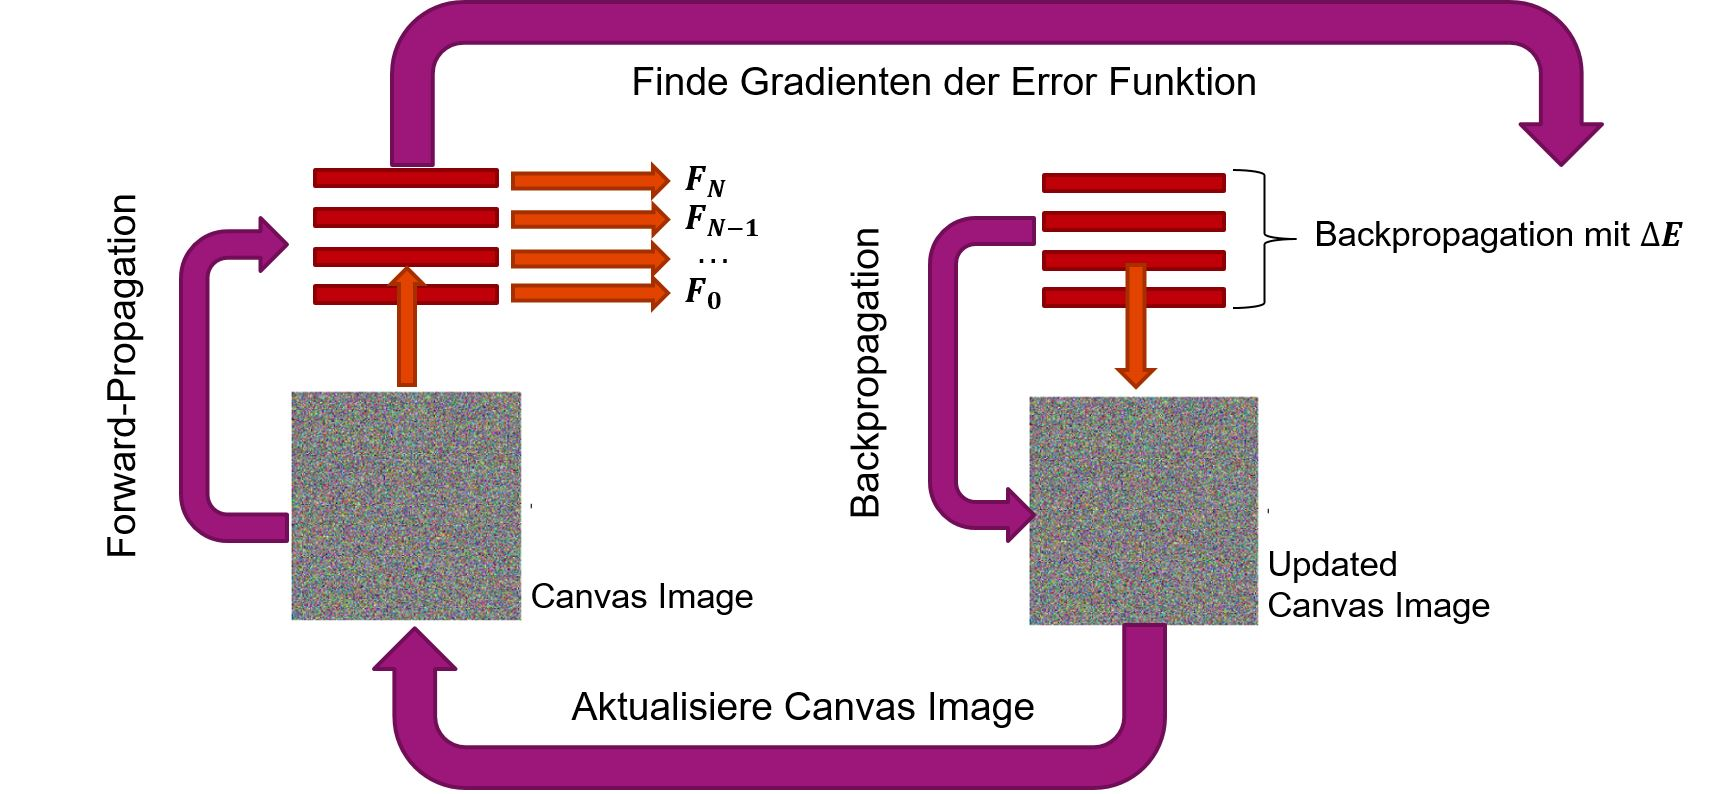
\includegraphics[width=\columnwidth]{Bilder/DeepStyle.jpg}
	\caption{Ablaufdiagramm des Deep Style Verfahrens.}
	\label{fig:DeepStyle}
\end{figure}
Abbildung~\ref{fig:DeepStyle} zeigt den schematischen Ablauf nach der erfolgreichen Initialisierung. Wie bereits erwähnt, beinhaltet das Canvas Image (CI) zufälliges Rauschen, welches während jeder Iteration in die Richtung von $\vv{GC}$ und $\vv{GS}$ transformiert wird. Das CI wird ebenfalls vorwärtspropagiert und mit den resultierenden Merkmalsvektoren $f$ aus jeder Schicht die Korrelation $G$ zwischen den einzelnen Merkmalsvektoren innerhalb einer Schicht ermittelt, wie in Gleichung~\ref{eq:DeepStyleCorr}. In dieser Gleichung ist $l$ die Anzahl Schichten im VGG. Dieser Schritt ist der erste zur Fehlerberechnung der Stilmerkmale in Gleichung~\ref{eq:DeepStyleErr}.
\footnotesize
\begin{equation}
G_{ij}^l= \frac{1}{2}\sum_{k=0} (\vv{f_{ik}}- \vv{f_{jk}})^2
\label{eq:DeepStyleCorr}
\end{equation}
\small
Im Anschluss wird mit diesen Korrelationen $G_{ij}^l$ jeweils pro Schicht die quadrierte Fehlerfunktion $F_l$ aus Gleichung~\ref{eq:DeepStyleCorrErr} berechnet. In diesem Fall bezeichnet $N$ die Anzahl der Merkmalsvektoren in einer Schicht und $M$ deren Größe. Für den gesamten Fehler des Stils $F_{style}$ werden alle $F_l$ wie in Gleichung~\ref{eq:DeepStyleErr} gewichtet aufsummiert.
\footnotesize
\begin{equation}
F_l= \frac{1}{2N_l^2M_l^2}\sum_{k=0}^N (G_{ij}^l- \vv{GS_{ij}^l})^2
\label{eq:DeepStyleCorrErr}
\end{equation}
\small
\footnotesize
\begin{equation}
F_{style}(SS,CI)= \sum_{k=0} w_l F_k
\label{eq:DeepStyleStyleErr}
\end{equation}
\small
Neben $F_{style}$ wird auch $F_{content}$ benötigt, doch dessen Berechnung ist weniger komplex. $F_{content}$ ist als simple quadrierte Fehlerfunktion aus $GC$ und den $f_{ij}$ der letzten Schicht definiert. 
\footnotesize
\begin{equation}
F_{content}(\vv{f_{GC}}, \vv{f})= \frac{1}{2}\sum_{i,j}(\vv{GC_{ij}}- \vv{f_{ij}})^2
\label{eq:DeepStyleContError}
\end{equation}
\small
Die gesamte Fehlerfunktion $F(SS,CS,CI)$ ergibt sich aus der gewichteten Summe von $F_{content}$ und $F_{style}$. Die beiden Gewichte $\alpha$ und $\beta$ ermöglichen dem Nutzer das Verhältnis zwischen Stil und Inhalt zu modifizieren und somit das Endergebnis seinen Vorstellungen anzupassen. 
\footnotesize
\begin{equation}
F (SS,CS,CI)= \alpha F_{con}+\beta F_{style}
\label{eq:DeepStyleErr}
\end{equation}
\small

\begin{figure}
	\flushleft
	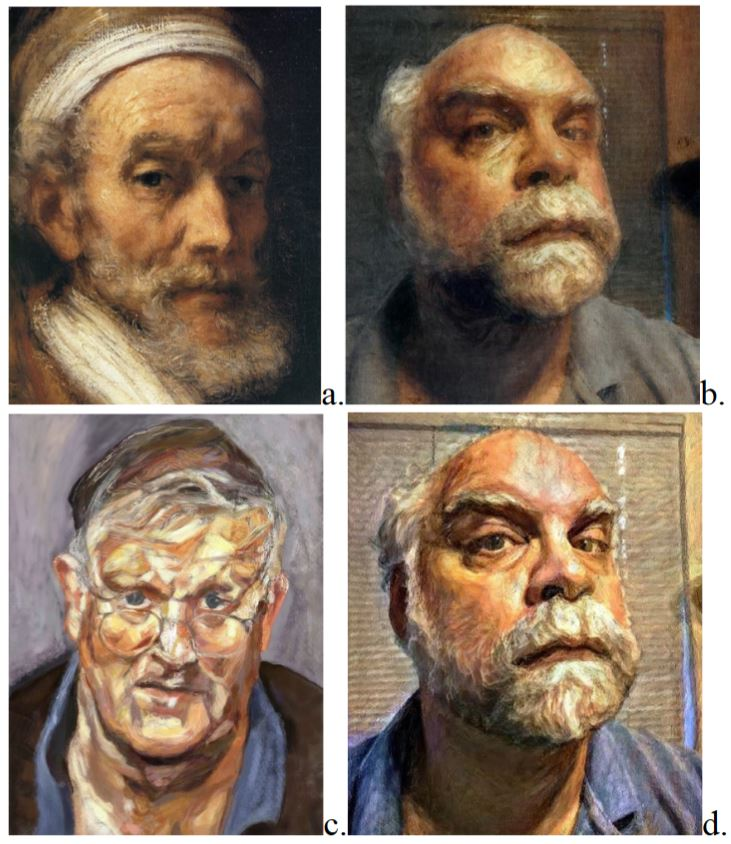
\includegraphics[width=\columnwidth]{Bilder/DeepStyleResults.JPG}
	\caption{Resultate des Deep Style Verfahrens~\cite{McCaigDG16}.}
	\label{fig:DeepStyleResults}
\end{figure}
Von $F(SS,CS,CI)$ wird, wie beim \textit{Deep Dream} Verfahren, auch der Gradient bestimmt um anschließend eine Rückwärtspropagation durchzuführen. Das weitere Ablaufschema gleicht dem des \textit{Deep Dream} und terminiert, wenn die Merkmalsvektoren von CI sich an die Initalisierungsvektoren von SS und CS angenähert haben.\\

Generell ermöglicht das \textit{Deep Style} Verfahren eine Stilsynthese ohne den Verlust von Bildinhalt (vgl. Abbildung~\ref{fig:DeepStyleResults}). Die Semantik und der Bildinhalt werden gut getrennt, wobei es unter Umständen vorkommt, dass die Trainingsdaten einen Einfluss auf das Endergebnis haben. Dieser Einfluss ist dennoch deutlich geringer als beim \textit{Deep Style} Verfahren~\cite{McCaigDG16}. Die Ergebnisse auf der rechten Seite der Abbildung haben die Semantik kohärent adaptiert ohne die Gesichtszüge der Person zu modifizieren. Die Farbwelt des SS wurde sinnvoll in die des CS transformiert. 

Die Gewichtung von Stil und Inhalt in $F (SS,CS,CI)$ ist skalierbar und ermöglicht dem Nutzer eine bessere Kontrolle über das Endergebnis. Generell wirken die Ergebnisse weniger zufällig und unabhängiger von den Trainingsdaten. In \cite{McCaigDG16} wurden neben den klassischen Gemälden auch photorealistische Bilder synthetisiert. Diese Resultate übertragen das Farbschema des SS nachvollziehbar auf das CS. Leider zur Zeit noch mit signifikanten Artefakten. An dieser Stelle besteht noch ein Optimierungsbedarf durch ein Pre- und Postprocessing oder einer geringeren Schichtanzahl. Dies könnte bei einer Übertragung des Farbschemas sinnvoll sein, da die Merkmalsvektoren weniger komplexe Strukturen enthalten.

Ein weiteres wichtiges Kriterium ist die Reproduzierbarkeit und die Kohärenz von ähnlichen Bildern. Um eine Reproduzierbarkeit zu gewährleisten muss stets von einem CNN mit der selben Initialisierung ausgegangen werden. Die Gewichtungen in einem CNN können durch ein erneutes Training nicht exakt reproduziert werden, deshalb ist es notwendig das CNN nach jeder erfolgreichen Synthese mit den selben Gewichtungen zu initialisieren. Bekannte Bibliotheken, wie zum Beispiel \textit{Caffe}~\cite{JiaCaffe}, bieten diese Möglichkeit an.
Die Kohärenz von aufeinanderfolgenden Bilder einer Videosequenz sollte möglich sein unter der Bedingung dass die Trainingsdaten einen äußerst geringen Einfluss haben und die Parameter $\alpha$ und $\beta$ konstant sind. Durch die naturgemäße konstante Beleuchtungssituation innerhalb einer Szenensequenz verfügen die CS über ähnliche Stilmerkmale und nur die Inhaltsmerkmale verändern sich teilweise. Letztere werden bekanntermaßen nur sehr gering modifiziert. Über die konkreten Unterschiede zwischen ähnlichen Bildern gibt es in der Literatur derzeit keine Aussagen.

Der Rechenaufwand steigt exponentiell mit der Bildauflösung. Derzeit ist eine Stilsynthese mit einer Auflösung von $512\times512$ Pixel für ein Einzelbild möglich, welche nicht ausreichend für die Videoproduktion ist. Aus diesem Grund ist die kostenintensive Nutzung von Renderfarms notwendig um eine ausreichende Qualität zu gewährleisten.

Mit vordefinierten Presets aus trainierten CNN und diversen CS ist auch eine Verwendung im Consumerbereich vorstellbar ohne dass der Nutzer detaillierte Kenntnisse über den Algorithmus besitzen muss. Generell ist das \textit{Deep Style} Verfahren sehr vielversprechend für die Videoproduktion und könnte mit einigen Optimierungen bei der Stilsynthese mit photorealistischen Bildern und der Nutzung einer Renderfarm einige Prozesse in der Postproduktion vereinfachen. 

\SubSection{Ausblick}
\todo[inline, color=red]{Vera} 
In der Zukunft kann das \textit{Deep Style} Verfahren für verschiedene Prozesse in der Postproduktion sinnvoll sein. Zunächst sei hier die qualitativ hochwertige und automatische Coloration und Texturierung von animierten Filmen ohne die aufwendige manuelle Texturierung von einzelnen 3D Objekten genannt. \\
Die Rekonstruktion und Restauration von verlorenen Filmmaterial, wie zum Beispiel \textit{Metropolis} von Fritz Lang ist auch vorstellbar. Da verlorene Szenen nachgestellt und im Anschluss an den Stil der verbliebenen Szenen angepasst werden könnten.\\
Auch eine individuelle Anpassung an den Geschmack und Stimmung des Nutzers von Filmen ist für \textit{Video-on-Demand} denkbar. Gerade die Farbgebung beeinflusst die Wahrnehmung des Zuschauers. So könnte zum Beispiel die Bedrohlichkeit eines Thrillers verschärft oder minimiert werden. Dasselbe gilt auch für Computerspiele, welche unter Umständen an Geschmack von jüngerem oder erwachsenem Publikum angepasst werden könnte.

\Section{Fazit} \label{Fazit}
\todo[inline, color=red]{Vera} 
Die vorgestellten Verfahren befinden sich noch am Anfang ihrer Entwicklung und erfordern noch weitreichende Optimierungen. Gerade der Ansatz zur Generierung von Szenen Dynamiken~\cite{VondrickPT16} scheint noch ausbaufähig zu sein. Dennoch bietet der Ansatz eine Grundlage für weitere Bemühungen in Richtung automatisierter Bewegtbildgenerierung. Zudem kann der Ansatz viele wichtige Erkenntnisse für die Weiterentwicklung von Videokodierungsverfahren liefern.

Das \textit{Deep Dream} Verfahren~\cite{DeepDream} scheint aufgrund nicht reproduzierbarer Ergebnisse und mangelnder Kontrolle durch den Nutzer für eine Verwendung in der Postproduktion uninteressant zu sein. Erfolgversprechender ist dagegen die Weiterentwicklung \textit{Deep Style}, welche die Semantik eines Bilder vom Inhalt trennen und übertragen kann. Nur die Synthese von photorealistischen Bildern enthält noch sichtbare Artefakte.

\textbf{Zusammengefasst zeigen die Verfahren, dass NN durchaus einen sinnvolle Verwendungszwecke in der Videoproduktion haben können und es lohnenswert ist, diese weiterzuverfolgen. Mit ihrer Hilfe könnten unter Umständen einzelne Arbeitsschritte in der Produktion und Postproduktion automatisiert werden, wenn die Verfahren weiterentwickelt und die Rechenkapazität weiter gesteigert wird. Lediglich die Automatisierung von kreativen Prozessen und der Generierung von vollständig neuen Ideen, wie zum Beispiel das Drehbuchschreiben, scheint zum jetzigen Zeitpunkt wenig vielversprechend.}


\newpage
\Urlmuskip=0mu plus 1mu\relax %Bricht Link in Bibfile um
\bibliographystyle{latex8} 
\bibliography{psm}

\end{document}

